



\section{Base FFLM}

Our CNN is constructed by extending a feed-forward language model (FFLM) with convolutional layers. In what follows, we first explain the implementation of the base FFLM and next, we describe the CNN that we study.

%~ Our baseline feed-forward language model (FFLM) is based on that of
%~ \newcite{bengio2006neural}, with a few modifications that much improve
%~ performance. The model is illustrated in Figure~\ref{fig:baseline} and
%~ works as follows. First, the input tokens are passed through a
%~ projection layer that fetches their associated vectors from a lookup
%~ table and concatenates them all together. This large vector is then
%~ fed to a fully-connected layer to produce a hidden layer. Next, and
%~ differently from the original model, a highway layer is
%~ used~\cite{srivastava2015highway}. 

Our baseline feed-forward language model (FFLM) is almost identical to the original model proposed by  ~\newcite{bengio2006neural}, with only slight changes to push its performance as high as we can, producing a very strong baseline. In particular, we extend it with highway layers and use Dropout as regularization. The model is illustrated in Figure~\ref{fig:baseline} and works as follows. First, each word in the input $n$-gram is mapped to a low-dimensional vector (viz. embedding) though a shared lookup table. Next, these word vectors are concatenated and fed to a highway layer ~\cite{srivastava2015highway}.
%The mechanism of highway layers is we can combine the non-linear affine transformation of an input layer with itself to create the output hidden layer. 
%Assuming the input and output of the highway layer is $H_I$ and $H_O$. The materials for a highway layer is a typical non-linear transformation $H$ and a transform gate $T$
%\begin{equation}
%\begin{aligned}
%H = f(H_I . W_h + b_h) \\
%T = (H_I . W_t + b_t)
%\end{aligned}  
%\end{equation}
%$W_h, b_h$ and $W_t, b_t$ are linear connected weights for the model, $f$ is a nonlinear function (ReLU in our work). Notably, the highway layer requires double the weights than a typical linear connected layer.
%The output of the highway layer is the combination of the transformed input and a part of the input carried away to the output. 
%\begin{equation}
% H_O = H \ast T + H_I \ast (1 - T)
%\end{equation}
Succinctly, highway layers improve the gradient flow of the network by computing as output a convex combination between its input (called the \emph{carry}) and a traditional non-linear transformation of it (called the \emph{transform}).
As a result, if there is a neuron whose gradient cannot flow through the transform component (e.g., because the activation is zero), it can still receive the back-propagation update signal through the carry gate.  %While deep feed-forward neural networks have not been shown to yield an important comparative advantage with respect to more shallow models~\cite{arisoy2012deep} ,
 We empirically observed the usage of a single highway layer to improve importantly the performance of the model. Even though a systematic evaluation for this model is beyond the scope of the current paper, our empirical results demonstrate that it is a very competitive one (see Section \ref{sect:exp}).    

%~ fed to a fully-connected layer to produce a hidden layer 
%~ works as follows
Finally, a softmax layer computes the model prediction for the upcoming word. We use ReLU for all non-linear activations and Dropout~\cite{hinton2012dropout} is applied between each hidden layer.%, which increase the regularisation capability of the network by randomly preventing forward activation of neurons during training. Notably, dropout is only applied to the fully connected components, thus having no effect on the convolutional layer .After the hidden layers, the output layer of the network is a softmax over the entire vocabulary. In experiments with large vocabularies, we factor the softmax layer with a hierarchical softmax~\cite{mikolov2011extensions} in order to improve the speed of the network. Specifically, the words are clustered into classes based on the unigram distribution frequency. After that, the network estimates the probability distribution over the class and another distribution over the words in that particular class. As a result, we can avoid large matrix computation. Finally, the activation function used in all experiments is ReLU. Not only can ReLU avoid gradient saturation, the activated neurons always have positive values, this facilitating the analysis of subsequent hidden layers




%~ Highway layers are
%~ $\dots$. \textbf{and Dropout? and Batch-norm?}. \textbf{Did we use HSM
  %~ for the experiments or not?} \gbt{Agree, we need info about
  %~ that}. Finally, a softmax layer yields the output of the network.

%~ \gbt{VERY IMPORTANT: Enlarge the font in all the figures (it should be approx.\ as large as
  %~ the one in the text). Add ``Hidden layer'' or simply ``H'' to the graph so
  %~ you can reference it in the text. What does the layer between the
  %~ highway layer and the softmax do?}

%~ \gbt{thanks for enlarging the font of the baseline model figure;
  %~ please enhance the font of figures 2 and 3, too}

%This section describes the general structure of our baseline model, which is illustrated in Figure~\ref{fig:baseline}. Essentially, we use the original architecture proposed in~\cite{bengio2006neural}. In the first layer, a lookup table is used to store the shared embedding space and query the context word vectors, which are in turn concatenate into one single context vector. The output layer is a softmax over the whole vocabulary, which can be factorized into an hierarchical softmax to reduce the complexity of the model~\cite{le2011structured,mikolov2011extensions}. Regarding the hidden layers, multiple hidden layers seem to have optimization problems~\cite{arisoy2012deep}. We empirically optimized the baseline network by using an additional highway layer~\cite{srivastava2015highway}, thus making the network similar to the lateral network in~\cite{devlin2015pre}. Furthermore, we use dropout~\cite{hinton2012dropout} to enhance regularisation for the model. 

%\textbf{Fixme: move later to the experimental part} Regarding the context size, we use $16$ words in the context for most of our experiments. Neural network language models, by their nature, can scale up the distribution for an arbitrary context size, which could be too sparse for count-based models~\cite{kneser1995improved}. It is notable that, the feed forward models in~\cite{hai2012measuring} do not benefit much from a context larger than $10$, yet the author only took into account the words in the current sentence. 
% Compared to the original architecture, our baseline model yield a better performance, due to the above mentioned extensions and better optimization ({\bf really? we just use SGD}) and regularisation, as shown in section~\ref{sect:exp}.

~ \begin{figure}[!t]
~ \centering
~ 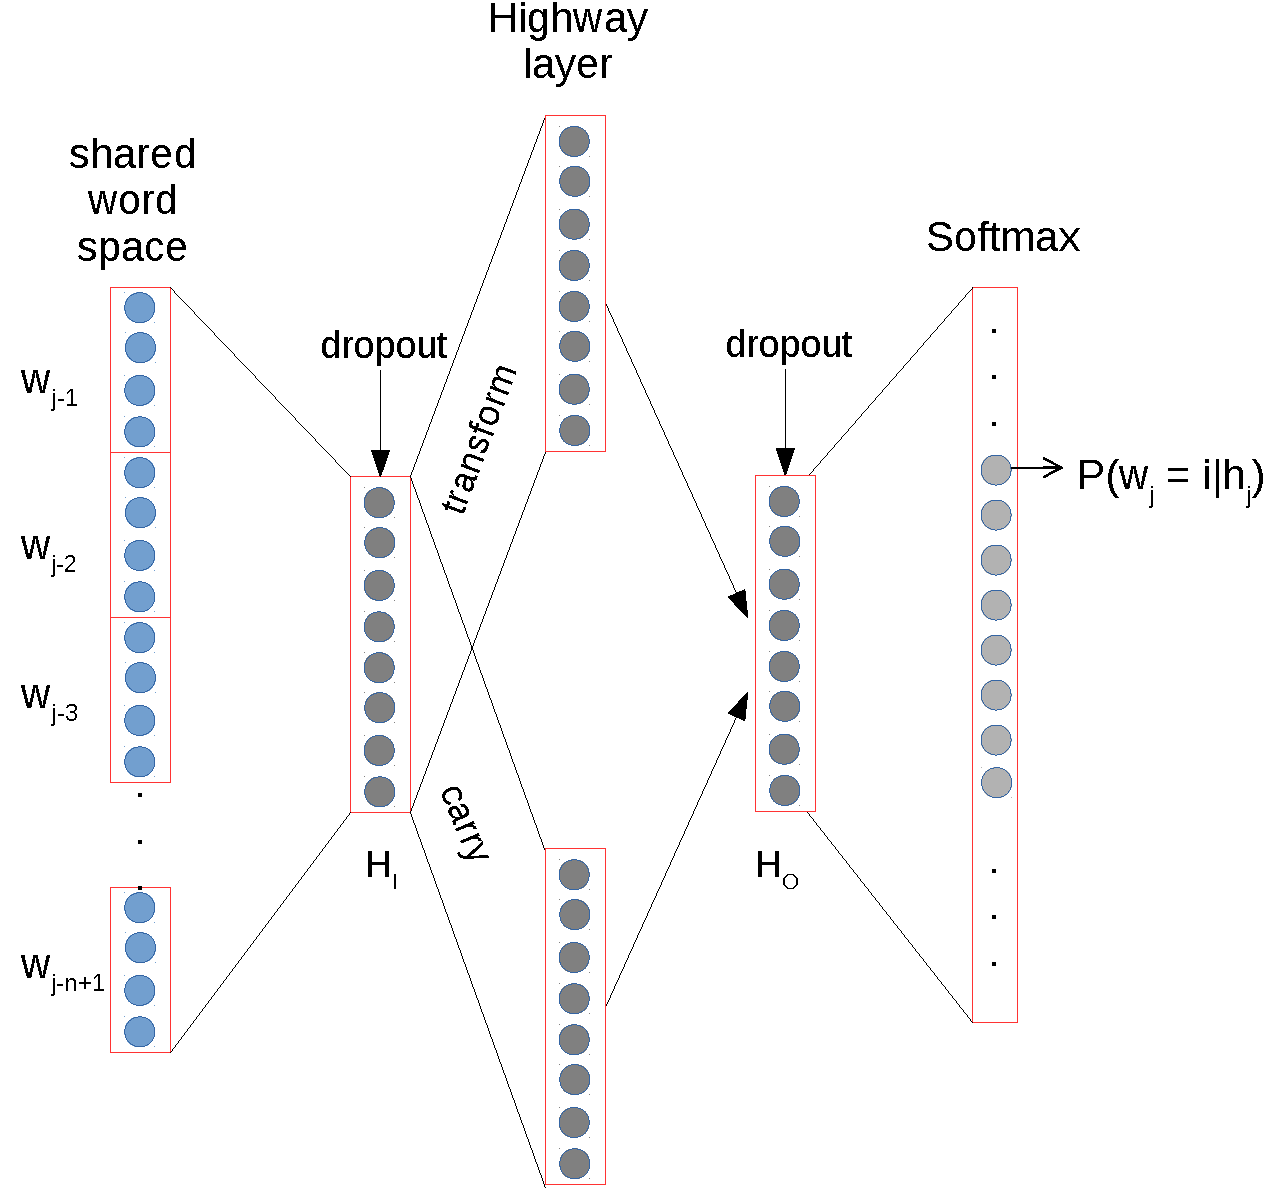
\includegraphics[width=\columnwidth/2]{figures/baseline.pdf}
~ \caption{Overview of baseline FFLM.}  
~ \label{fig:baseline}
~ \end{figure}
%\begin{figure*}[!t]
%\begin{minipage}{.5\linewidth}
%
%\centering
%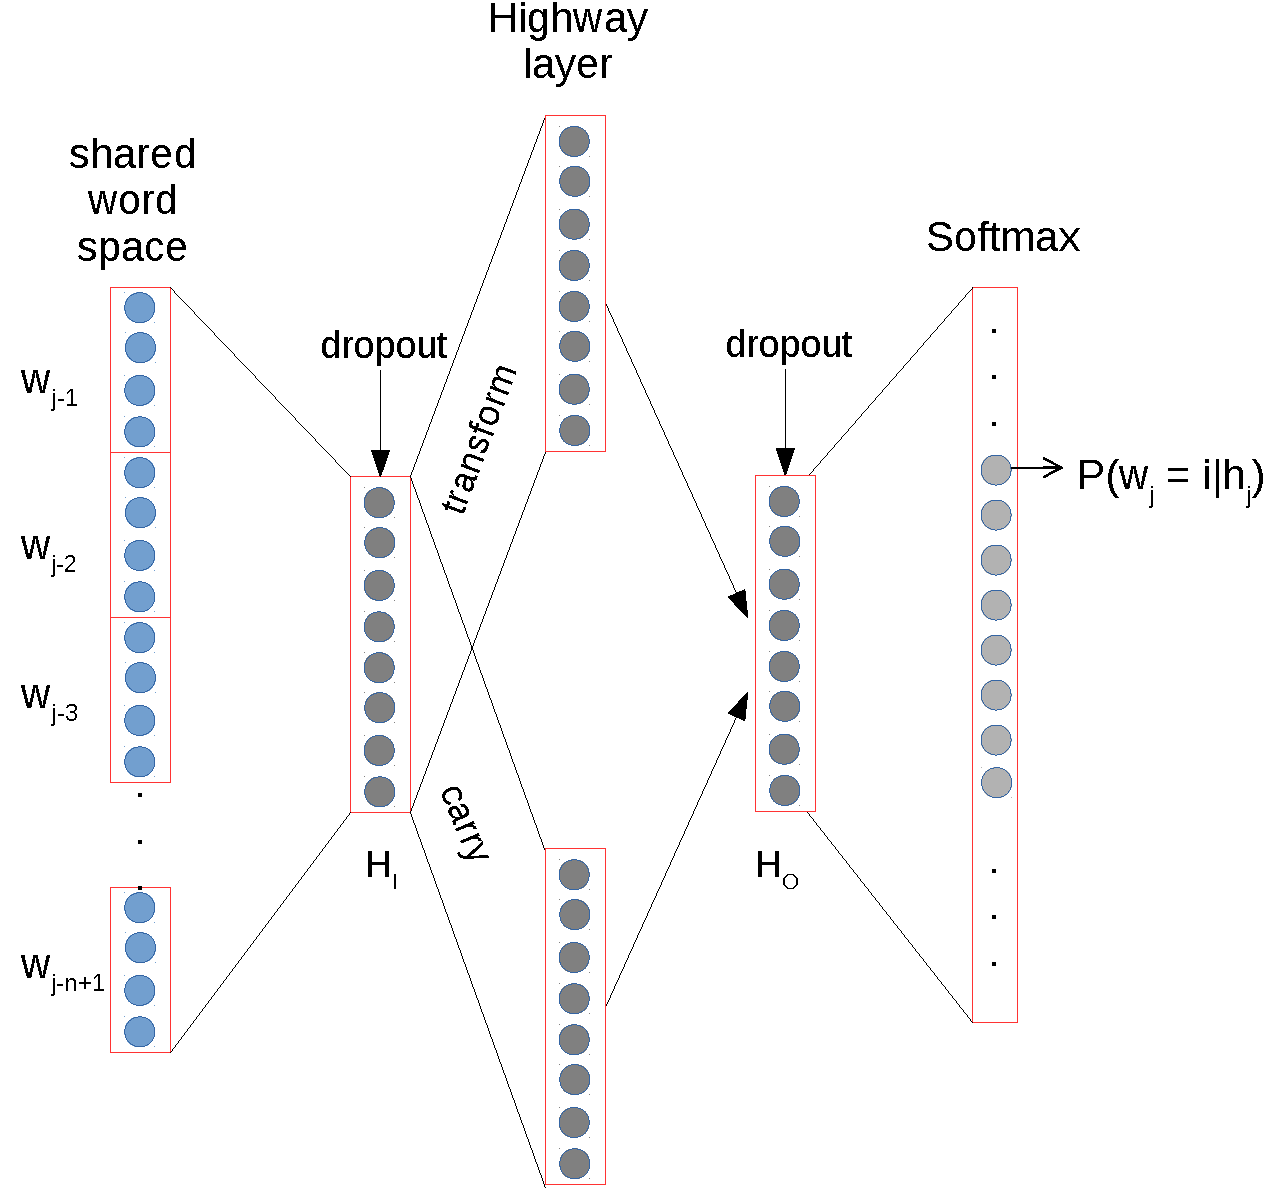
\includegraphics[width=1\linewidth]{figures/baseline.pdf}
%\caption{Overview of baseline FFLM.}  
%\label{fig:baseline}
%%~ \end{figure}
%\end{minipage}
%\begin{minipage}{.5\linewidth}
%%~ \begin{figure}[!t]
%\centering
%\vspace*{15mm}
%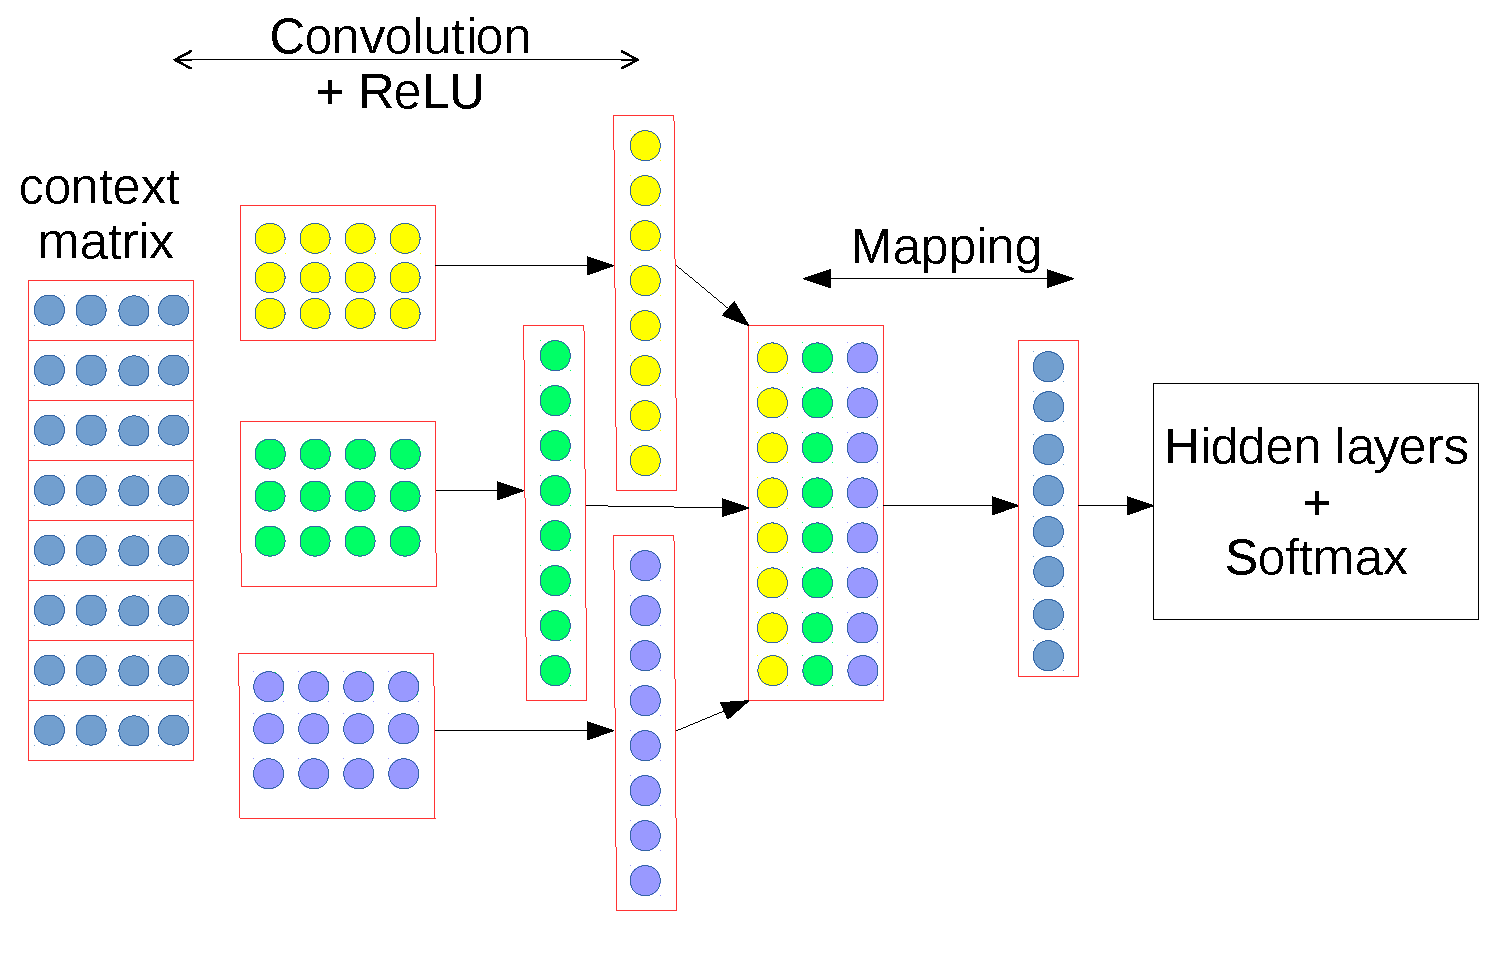
\includegraphics[width=1\linewidth]{figures/convolution.pdf}
%\vspace*{4mm}
%\caption{CNN layer on top of the context matrix.}  
%\label{fig:simpleconv}
%\end{minipage}
%\end{figure*}

\section{CNN and variants}

The proposed CNN network is produced by injecting a convolutional layer right after the words in the input are projected to their embeddings (Figure \ref{fig:simpleconv}). Rather than being concatenated into a long vector, the embeddings $x_i \in \mathbb{R}^k$ are concatenated transversally producing a matrix $x_{1:n}  \in \mathbb{R}^{n \times k}$, where $n$ is the size of the input and $k$ is the embedding size.  %Consequently, we minimally change the network structure and the number of parameters and the network only learns word patterns through the convolutional kernels.
%Similarly to \newcite{collobert2011natural} and
%\newcite{kim2014sentence}, we utilize a time-delayed
%network~\cite{waibel1989phoneme} where the input vectors are convolved
%through various learned kernels.
%
%The computation is done as follows. Let $x_i \in \mathbb{R}^k$ be the
%vector associated with the $i$-th input context word. First, all these
%vertical vectors are concatenated horizontally leading to a matrix
%$x_{1:n}$ of size $k \times n$:
%\begin{equation}
%x_{1:n} = x_1 \oplus x_2 \oplus \dots \oplus x_n
%\end{equation}
% In which, $x_{1:n}$ is a matrix of size $k \times n$, which is
% different to the long context vector in the baseline model.
This matrix is fed to a time-delayed layer, which convolves a
sliding window of $w$ input vectors centered on each word vector using a
parameter matrix $W \in \mathbb{R}^{w \times k}$. Convolution is performed
by taking the dot-product between the kernel matrix $W$ and each
sub-matrix $x_{i-w/2:i+w/2}$ resulting in a scalar value for each position $i$ in input context. This value represents how much the words encompassed by the window  match the feature represented by the filter $W$. A ReLU activation function is applied subsequently so negative activations are discarded. %In summary, we compute:
%\begin{equation}
%y_i = f(W \ast x_{i:i+w-1} + b)
%\end{equation}
%where $W$ and $b$ are learnable parameters of the convolutional
%kernel, and $f$ is a nonlinear function. A specific kernel can be %seen
%as a detector for a particular feature and the output $y_i$ can be
%seen as an indication for whether the feature is present or not at the
%current time step. 
This  operation is repeated multiple times using
various kernel matrices $W$,  learning different features independently. Here we tie the number of learned kernels to be the same as the embedding dimensionality $k$. Thus, the output of this stage will be another matrix of dimensions $n \times k$ containing the activations for each kernel at each time step.

%Typically, there are four main hyper-parameters involved in deciding
%the output sizes of the convolutional neural networks. The number of
%kernels indicates the {\bf depth} (number of features to be detected)
%of the output, while the {\bf kernel size}, the {\bf stride} (the distance
%between two convolutional steps), and {\bf zero paddings} at the beginning
%and the end of the input decides the number of convolutional steps.  In order to
%simplify the experiments, we assume that the number of convolutional
%features is proportional to the embedding dimensionality, and fix the
%number of kernels to be equal to the latter ($k$). The stride is kept
%to $1$ and zero padding is added with respect the the kernel width
%(number of words in one step). As a result, the size of the
%convolutional output is $n \times k$, which has the same neurons as
%the input embeddings. 
%
Next, we add a batch normalization stage immediately after the convolutional output, which facilitates learning by addressing the internal covariate shift problem and regularizing the learned representations~\cite{DBLP:journals/corr/IoffeS15}. 

%~ \gbt{Which is the third hyper-parameter?}


%~ For our experiments, we fix the number of kernels to be equal to the embedding dimensionality $k$ to simplify the number of hyper-parameters. Moreover, with zero-padding at the beginning and the end of {\bf ????}

%~ The output of this temporal convolution layer is thus a matrix with size $n \times m$ {(\bf check: $n \times k$?)}, in which $m$ {\bf check: $k$?} is the number of kernels. 

Finally, this feature matrix is directly fed into a fully connected
layer that can project the extracted features into a lower-dimensional
representation. This is different from previous work, where a
max-over-time pooling operation was used to find the most activated
feature in the time series. Our choice is motivated by the fact that
the max pooling operator loses the specific position
where the feature was detected, which is important for word prediction.
%A positive
%side-effect is that the fully connected layer essentially makes the
%subsequent parts of the network identical to the baseline model, thus
%simplifying the comparison. In particular, we can set the CNN model to
%have almost the same number of weights as the baseline. 

After this initial convolutional layer, the network proceeds identically to the FFNN by feeding the produced features into a highway layer, and then, to a softmax output.
%Also, because
%the structures are similar we can recycle hyper-parameter values from
%the baseline to the CNN models. 

This is our basic CNN architecture. We also experiment with three
expansions to the basic model, as follows. First, we generalize the CNN by
extending the shallow linear kernels with deeper multi-layer
perceptrons, in what is called a Network-in-Network ({\bf NIN})
structure~\cite{lin2013network}. %Since deeper networks have better
%representation potential, the NIN structure 
This allows the network to produce non-linear filters, and it has achieved
state-of-the-art performance in object recognition while reducing the
number of total layers compared to other mainstream networks. Concretely, we implement NIN networks by using another convolutional layer with a $1 \times 1$ kernel
on top of the convolutional layer output. Notably, we do not include the global pooling layer in the original work. 

Second, we explore stacking convolutional layers on top of each other (Multi-layer CNN or \textbf{ML-CNN}) to connect the local features into broader regional representations, as commonly done in computer
vision. While this proved to be useful for sentence
representation~\cite{Kalchbrenner2014conv}, here we have found it to be rather harmful for language modeling, as shown in Section~\ref{sect:exp}.


% In our structure, since
% the output of the convolutional layer has the same dimensions as the
% embedding inputs, it is intuitive to apply other convolutional
% layers.
Finally, we consider combining features learned through different kernel sizes (\textbf{COM}), as depicted in Figure \ref{fig:combine}. For example, we can have a combination of kernels that learn filters over 3-grams with others that learn over 5-grams. This is achieved simply by applying in parallel two or more sets of kernels to the input and concatenating their respective outputs~\cite{kim2014sentence}.%, in which the max-pooling outputs are concatenated, we introduce \textbf{Convolutional Blocks} (Figure~\ref{fig:combine}) that operate in parallel. Each block independently scans the context matrix with a different kernel size $w$. After mapping the convolutional features to lower dimensions, we concatenate them into a single one. Notably, by doing so we also increase the size of the hidden layers which results in the rise of parameters in the output layer.  


~ \begin{figure}[!t]
	\centering
~ 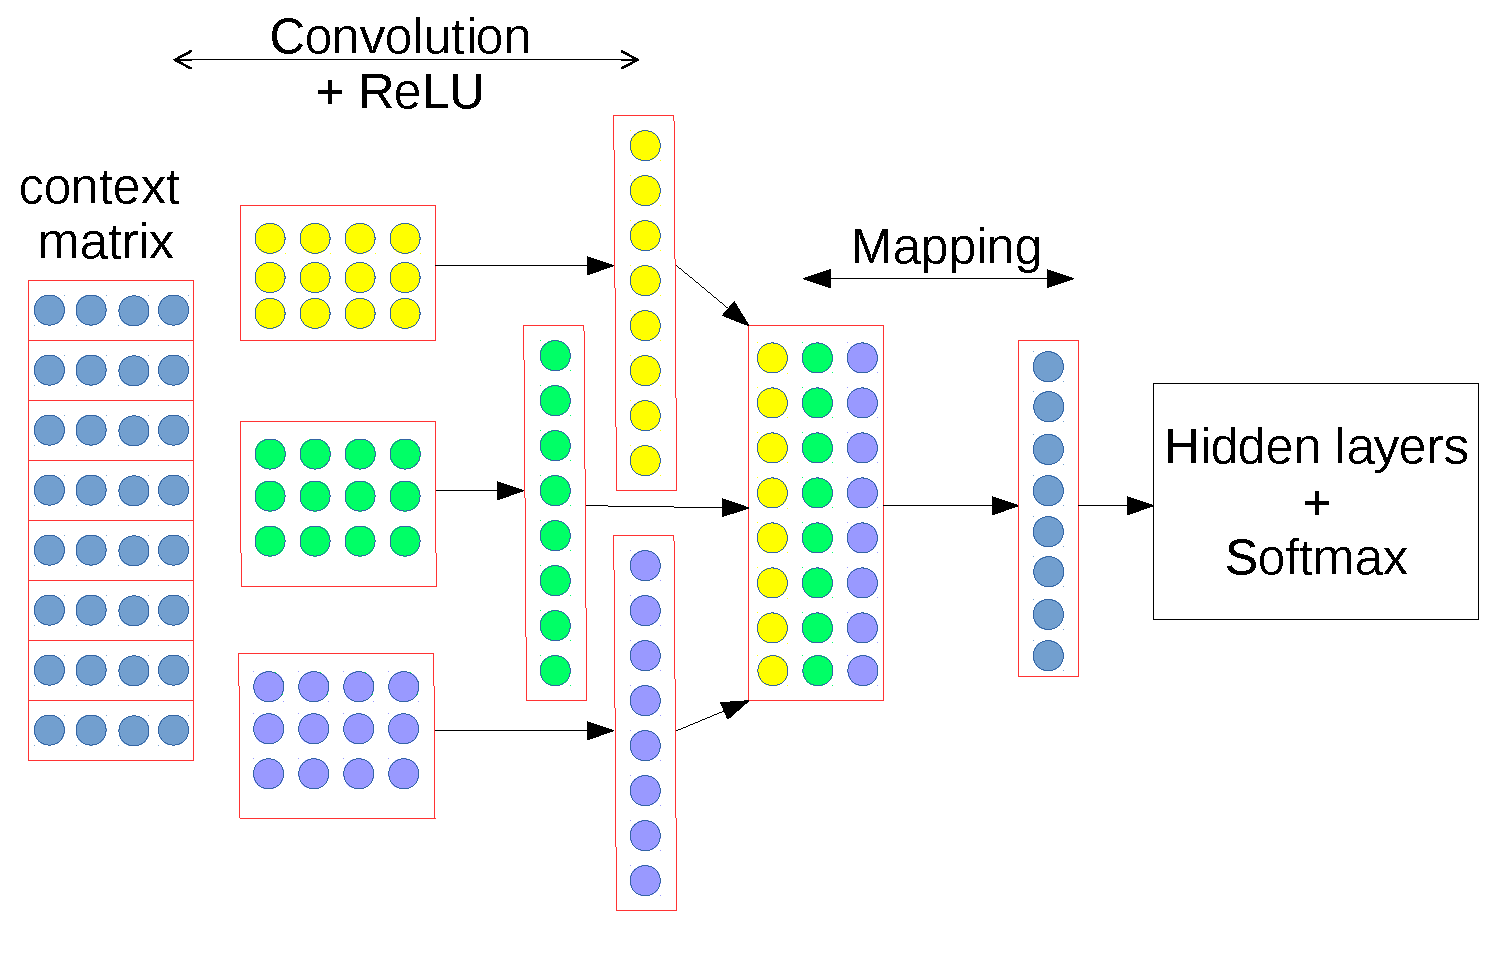
\includegraphics[width=\columnwidth*3/4]{figures/convolution.pdf}
~ \caption{Convolutional	 layer on top of the context matrix.}  
~ \label{fig:simpleconv}
~ \end{figure}
%
\begin{figure}[!t]
\centering
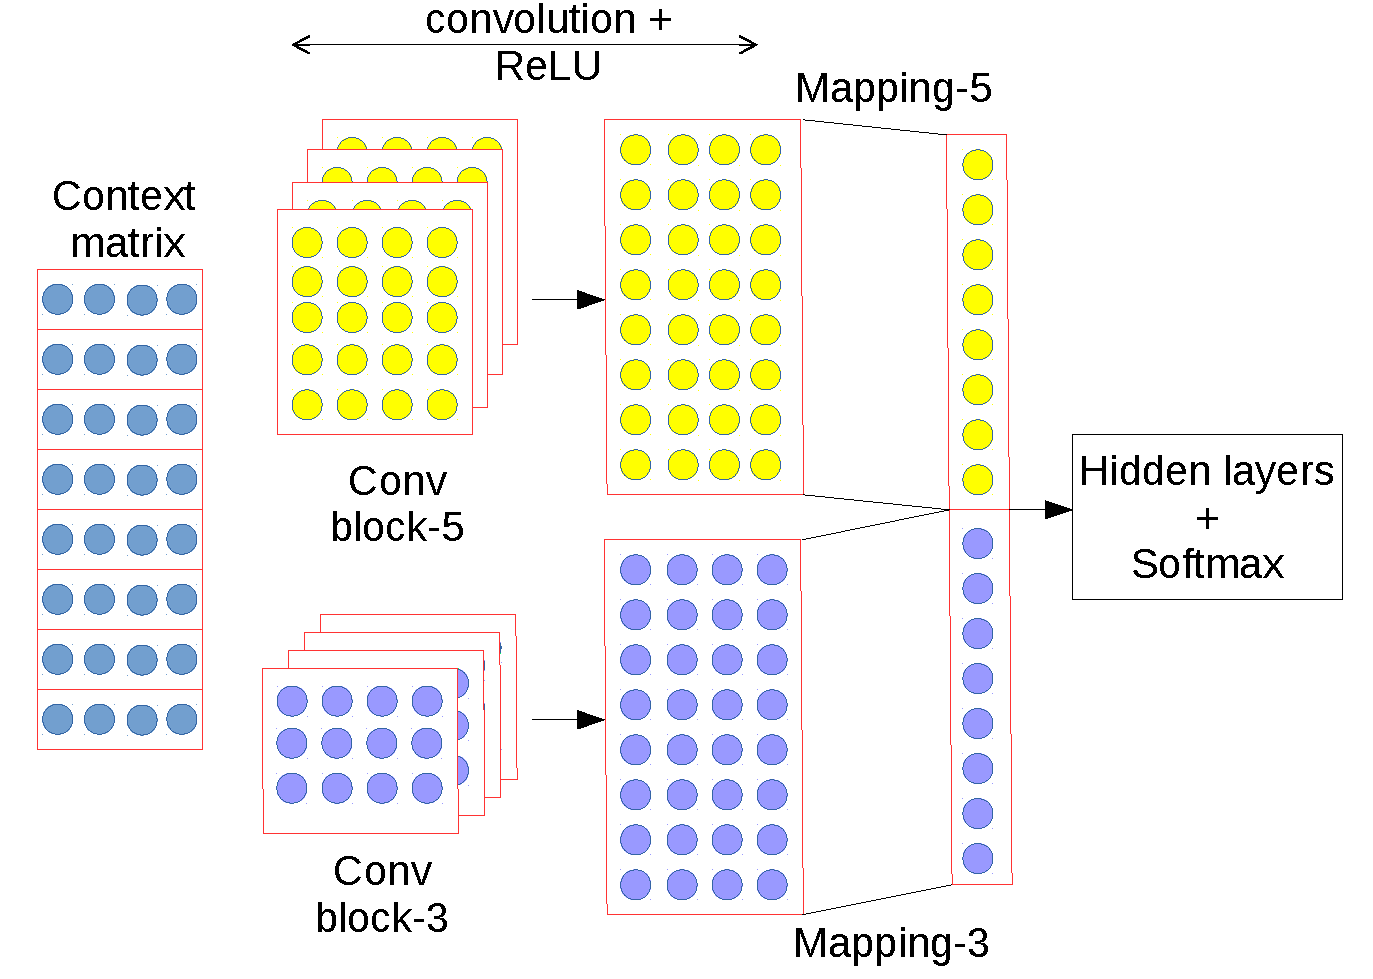
\includegraphics[width=\columnwidth*3/4]{figures/combine.pdf}
\caption{Combining kernels with different sizes. We concatenate the outputs of 2 convolutional blocks with kernel size of $5$ and $3$ respectively.}  
\label{fig:combine}
\end{figure}